%% Doc Props
\documentclass[11pt,a4paper]{article}
\usepackage[utf8]{inputenc}
\usepackage[english]{babel}

% Packages
\usepackage{
  titlesec,
  %tikz,
  textcomp,
  fixltx2e,
  color,
  fullpage,
  graphicx,
  afterpage,
  float,
  parskip,
  xfrac,
  gensymb,
  mathtools,
  pdfpages,
  etoolbox,
  hyperref
}
\usepackage[nottoc,section,numbib]{tocbibind}
%\usepackage[europeancurrents,europeanvoltages,europeanresistors,europeaninductors,smartlabels]{circuitikz}
%\usepackage{pgfplotstable}
%\pgfplotsset{compat=1.12}
%\usetikzlibrary{calc,matrix,positioning,arrows,shapes,trees,plotmarks,decorations.markings}
\usepackage[font={small,it}]{caption} %% Italics in captions

% PDF props
\hypersetup {
  bookmarks=true,              % show bookmarks bar?
  unicode=true,                % non-Latin characters in Acrobat’s bookmarks
  pdftoolbar=true,             % show Acrobat’s toolbar?
  pdfmenubar=true,             % show Acrobat’s menu?
  pdffitwindow=false,          % window fit to page when opened
  pdfstartview={FitH},         % fits the width of the page to the window
  pdftitle={G41 Project Report},                 % title
  pdfauthor={Oscar Petersson}, % author
  pdfsubject={TSIU03 Project Report},          % subject of the document
  pdfkeywords={TSIU03,Project,Report}          % list of keywords
  pdfnewwindow=true,           % links in new window
  hidelinks,                   % hide links (removing color and border)
  linktoc=all,                 % parts of TOC made into links    
}
\urlstyle{same}

% More Props
\graphicspath{{./fig/}}
\graphicspath{{../Designspec/fig/}}

% Comfy Command Redefinitions
\newcommand{\bve}{\begin{verbatim}}
\newcommand{\itb}{\begin{itemize}}
\newcommand{\ite}{\end{itemize}}
\newcommand{\tb}{\textbackslash}
\newcommand{\citeD}{\emph{Design Specification \cite{design}}}
\newcommand{\citeR}{\emph{Requirement Specification \cite{reqspec}}}
\newcommand{\citeF}{\emph{First Presentation \cite{pres}}}
\newcommand{\citeP}{\emph{Project Plan \cite{plan}}}
\newcommand{\citeM}[2]{\texttt{#1.vhd} \cite[line #2]{#1}}

%% First Page Information
\author{Niklas Blomqvist, Philip Johansson, Matteus Laurent, Johan Levinsson, Oscar Petersson, Erik Peyronson}
\title{Group 41 - Project Report}
\date{\today}
\newcommand{\course}{System Design - Project, HT15}
\newcommand{\coursenumber}{TSIU03, Linköpings universitet}
\newcommand{\programme}{Högskoleingenjörsutbildning i datateknik, 180 hp}
\newcommand{\examiner}{Petter Källström}
\newcommand{\institution}{Department of Electrical Engineering (ISY)}
\newcommand{\reptype}{Project Report}

%%% Document %%%
\begin{document}

\setcounter{secnumdepth}{3}
\setcounter{tocdepth}{3}

%% Custom titlepage, empty backside, do not use with \maketitle
\pagestyle{empty}
  \makeatletter\begin{center}~\vfill
  \Large{\@author}\vskip .3cm
  \textbf{\LARGE{\@title}}\vskip .2cm
  \large{\programme}
  \vfill
\end{center}
\reptype{} - \@date\hfill Supervisor:\\
\textbf{\course}\hfill\examiner\\
\coursenumber\hfill\institution
\makeatother
\newpage

%% Table of Contents
\addtocontents{toc}{\protect\hypertarget{toc}{}}
\tableofcontents\label{sec:toc}
\addtocontents{toc}{\protect\thispagestyle{empty}}
\cleardoublepage
% Call First File Branch
%
%\chapter{Vad dokumentet ska innehålla:} % Detta ska bort innan inskick
%The entire Design Spec should be 5-7 pages

\begin{itemize}
\item Now you are the engineers who receive the requirement specification. What you have to do is to propose a solution that fulfills the requirements of the system.
\item Contrary to the requirements specifications, now you have to think about HOW you are going to meet  the requirements.
\item The design specification must describe the entire system. Think about the main blocks that your system will have, the functionality of each block and the interaction between them, i.e., which information the have to send to each other. Explain the functionality of the blocks and their interaction from a signal processing point of view, i.e., how the audio, video, etc. are processed in each block and which infomation is transmitted between blocks. You can provide som equations to show the algorithms that are applied. Note that this is very different from providing the hardware interfaces between the blocks.
\item Later, think about the difficulties that you will find in hardware and the hardware limitations (timing, bandwidth, word length, etc.) and check that your design is viable. Some calculations may be necessary. For instance, if a requirrement says that the system must be able to delay the audio signal one second, you will probably think of using a memory in order to meet the requirement. Then you should make some calculations to check how big the memory must be and if it fits in the FPGA or if you need to use an external memory.
\item The design specification must be described from the system level. Please, avoid details that are not relevant at that level. Also, make sure that the person who reads the document can get a clear idea of the entire system.
\item As a result, the design specification must be a technical proposal that shows that you have analyzed the problem and found the difficulties that you will face, and provides a first approach to the solution. A good approach for writing the design specification is to present a block diagram of the system, provide a high-level description (at signal processing level) about the functionality of each block and how the blocks interact, and show which requirements present challenges and how you will solve them in hardware.
\end{itemize}

\section{Layoutstandarder}
Läs README:n i ../Projektrapport/ först och främst. Jag har strukturerat det hela genom att ha varje chapter och section i en fil med motsvarande namn, och nya borde inte behövas. Referera till bilder, avsnitt etc. på adekvat sätt med\texttt{\textbackslash{}ref} (ger kapitelnummer eller figurnummer) och \texttt{\textbackslash{}pageref} (ger sidnummer).
Hänvisningar inom parentes sätts ej kursivt, i löptext anges de enligt (ta gärna en titt i description.tex):
\begin{verbatim}
  \emph{<Typ> \ref{ref:name}: Name}
\end{verbatim}

Jag föreslår även att vi använder oss av \verb#\verb+name+# för att markera namn på moduler, signaler, etc.

Förhoppningsvis har ni vid det här laget bekantat er med min \LaTeX{}-guide, men har ni frågor är det bara att hojta. Använd gärna emacs för att redigera dokumenten då det har stöd för uppmärkning av \LaTeX{}-syntax.

Får jag igång SSH:n till burken därhemma via skolans burkar ska jag försöka hålla autokompileringen vid liv under dagen, men jag garanterar inget.
                 % och likaså denna rad

\chapter{Introduction}\label{ch:introduction}
\setcounter{page}{1}

%%Första sidan
\begin{frame}
	\frametitle{Introduction}
		\begin{itemize}
			\item Audio signal processing
			\item 	Signal level indicator	
			\item Our own flavor:
				\begin{itemize}
				\item Background image
				\item Graphic scales for L/R input/output channels
				\item Class-D amplifier
			\end{itemize}
		\end{itemize}
\end{frame}


%%Andra sidan
%\begin{frame}
%\frametitle{UI}
%	\begin{itemize}
%		\item Volume
%			\begin{itemize}
%				\item Eleven different stages, exclusive mute.
%			\end{itemize}
%		\item Balance
%		\begin{itemize}
%				\item Seventeen different stages.
%			\end{itemize}
%		\item Mute
%		\item Peak level indicator
%	\end{itemize}
%\end{frame}


%Bild över UI
%%Tredje sidan

\begin{frame}
	\frametitle{UI}
	  \begin{figure}[h]
    \centering 
    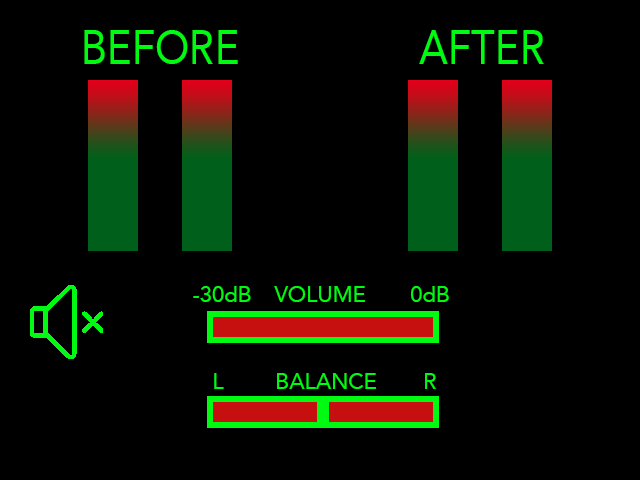
\includegraphics[scale=0.80]{UI2.png} 
       \label{UI}
  \end{figure}
\end{frame}




\chapter{System Level Description}\label{ch:description}
\emph{System Level Description (Block diagram + description of 1 to 2 pages).}

\emph{(Make sure that your description justifies how the Requirements of your system are met, especially those which are not obvious.)}

%% Remove the text above

This chapter will describe the system main blocks, the functionality of each of them, and the interaction between each block. Presented below (Figure \ref{fig:overview}) is a graphical overview over the system and its first layer of modules. A high resolution version is also included in \emph{Appendix \ref{app:overview}: System Overview}.

\begin{figure}[H]
  \centering
  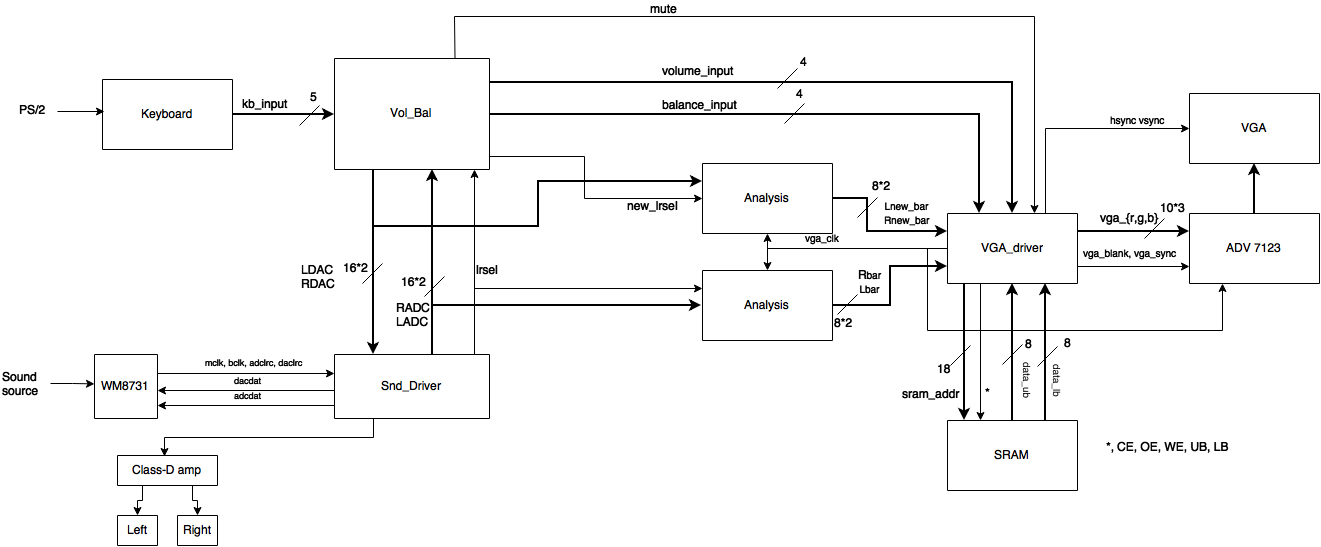
\includegraphics[scale=.18]{overview}
  \caption{A graphical overview of the system's first module layer.}
  \label{fig:overview}
\end{figure}

\section{Keyboard}\label{sec:keyboard}
The user interacts with the system through a PS/2-connected keyboard. The keyboard is then handled by the module \verb?Keyboard? which reads the scan codes, matches these against a \emph{one hot encoded} preset which makes up the \verb?kb_input? signal passed to \verb?Vol_Bal?.

The module inputs are \verb=PS2_DAT=, \verb=PS2_CLK=, \verb=clk= and \verb=rstn= which are used to shift in the scan code and compare the result with the preset, resulting in \verb=kb_input= --- a 2-bit unsigned value indicating if either of the arrow keys have been released. \verb=Vol_Bal= will then use this signal to adjust the volume and balance level. The Up/Down arrow keys controls the volume, and the Left/Right arrow keys controls the stereo channel balance.


\section{Snd\_Driver}\label{sec:snddriver}
The \verb?Snd_Driver? module is an audio signal coder/decoder. It translates the signal between a parallel format and a bit serial format. The parallel format is sent to the \verb?Vol_Bal? module which processes the sound and sends it to the class-D amplifier. The bit serial format is used by the WM8731 chip and the amplifier. This module will be a complete copy of the module used in \emph{Laboration 4}. In this case the module \verb?Vol_Bal? will replace and expand the \verb?Application? used in that laboration.

\begin{figure}[H]
  \centering
  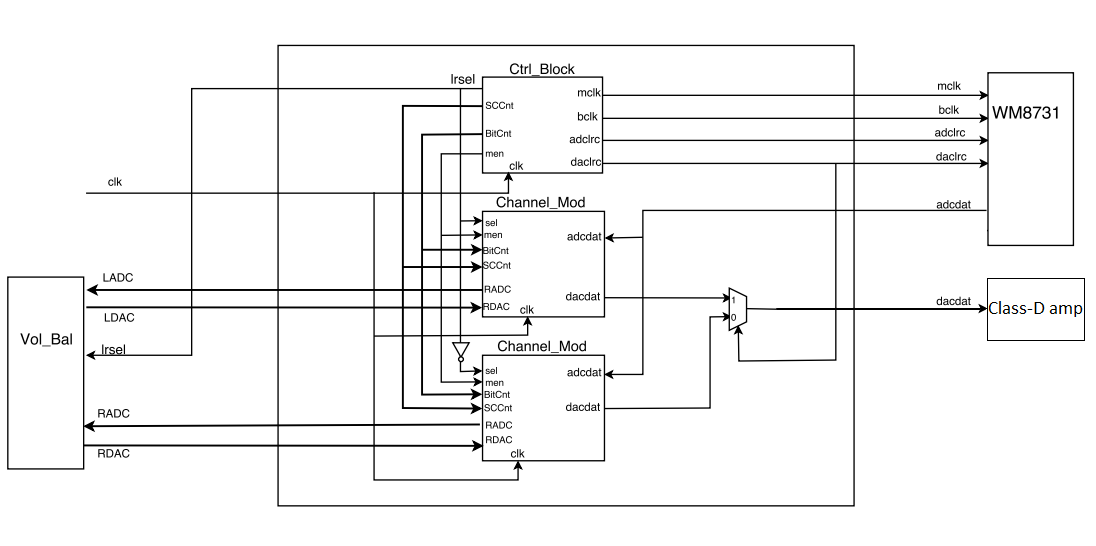
\includegraphics[scale=.40]{snddriver}
  \caption{The \texttt{Snd\_Driver} schematic, as seen in Lab 4, Audio Codec.}
  \label{fig:sndDriver}
\end{figure}


\section{Vol\_Bal}\label{sec:volbal}
The Volume/Balance module (\verb=Vol_Bal=) acts as the hub for processing incoming digital audio signals, forwarded from WM8731 via the \verb=Snd_Driver= module. As such, \verb=Vol_Bal= also keeps internal registers in the module \verb=Current_Vol_Bal= that holds volume (4-bit unsigned) and balance levels (4-bit signed), as well as a mute signal (std\_logic). These registers update via the one-hot coded input signal \verb=kb_input= applied by the \verb=Keyboard= module. Consequently, the values they hold are not only used as signals (\verb=i_volume_lvl=, \verb=i_balance_lvl=, \verb=i_mute=) for the internal submodule that process the \verb=LADC= and \verb=RADC= inputs, but also as module outputs connected to the \verb=VGA_Driver= so that they can be rendered on the screen.

\begin{figure}[h]
  \centering
  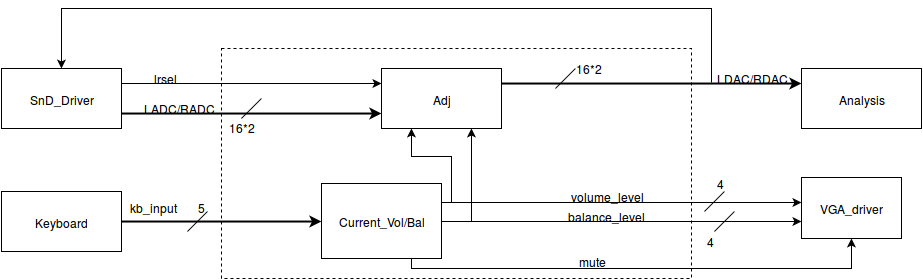
\includegraphics[width=16cm]{volbal}
  \caption{An overview of the Vol\_Bal module's internal workings.}
  \label{fig:vol_bal}
\end{figure}

The main function of the Volume/Balance module is to make requested adjustments to incoming values \verb=LADC= and \verb=RADC=, which represent measured amplitudes of the sound signal at distinct times. The sound will be adjusted for volume and balance by the functions:

\verb=   =$$A_{l\_new} = A_{l\_old} \cdot (1/\sqrt{2})^{n + m}\qquad\ ,\ m = 0\ for\ m < 0$$
\verb=   =$$A_{r\_new} = A_{r\_old} \cdot (1/\sqrt{2})^{n + |m|}\qquad,\ m = 0\ for\ m > 0\ ,$$

where $A$ is the amplitude, $n$ the volume level and $m$ the balance. \verb=lrsel= is used as a control signal for selecting the channel and the correct function. Resulting outputs \verb=LDAC= and \verb=RDAC= are forwarded to \verb=Snd_Driver= and to one instance of the \verb=Analysis= modules.

Ultimately, the user have the ability to digitally adjust the input sound by decreasing the volume in 3 dB decrements, down to -30 dB, and additionally regulate balance bias by further reducing volume by up to another 15 dB on a single left/right audio channel. There is also a mute function which is conveyed by \verb=kb_input=. When active, the register driving the \verb=mute= signal essentially blanks any $A_{new}$ values on the \verb=LDAC/RDAC= outputs.




\section{Analysis}\label{sec:analysis}
\begin{frame}
  \frametitle{Analysis}
	\begin{itemize}
		\item Analyzes incoming samples, low-pass filtering them.
		\item Output in form of a natural number, which determines the height of the bars.
		\item Updates in synd with vsync.
		\item Both left & right channel separately.
	\end{itemize}
\end{frame}

\begin{frame}
  \frametitle{Analysis}
	\begin{figure}[h]
		\centering
			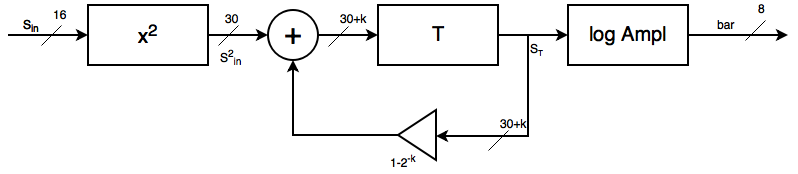
\includegraphics[width=16cm]{lowpass}
			\caption{The low-pass filter. $k$ is chosen by the approximation $\frac{1}{10}\mathrm{\ s} = 2^k\cdot\frac{1}{48800}\Rightarrow 2^k=4880\approx 2^{12}\Rightarrow k = 12 $}
			\label{fig:lowpass}
\end{figure}
\end{frame}


\section{VGA\_driver}\label{sec:vgadriver}
The \verb+vga_drive+ module exists to handle the rendering of a 640x480 resolution image on the screen. 
The image that is supposed to be rendered consists of a background image previously 
stored in the SRAM consisting of pre filled bars that within the module will be blanked
out according to the input stimuli, which will give the appearance of bars being filled 
to different levels.   

To render an image on the vga screen you need five main signals. Three analog color channels (red, green and blue)
and two signals for synchronization hsync and vsync. The image is rendered pixel by pixel line by line using
a horizontal sweep pattern which is reset by the two sync signals. If a color is set when the sweep resets
arbitrary patterns can occur and therefore the signal has to be blanked during the reset phase.

The module \verb+vga_drive+ has four input signals described in 

\begin{figure}[h]
        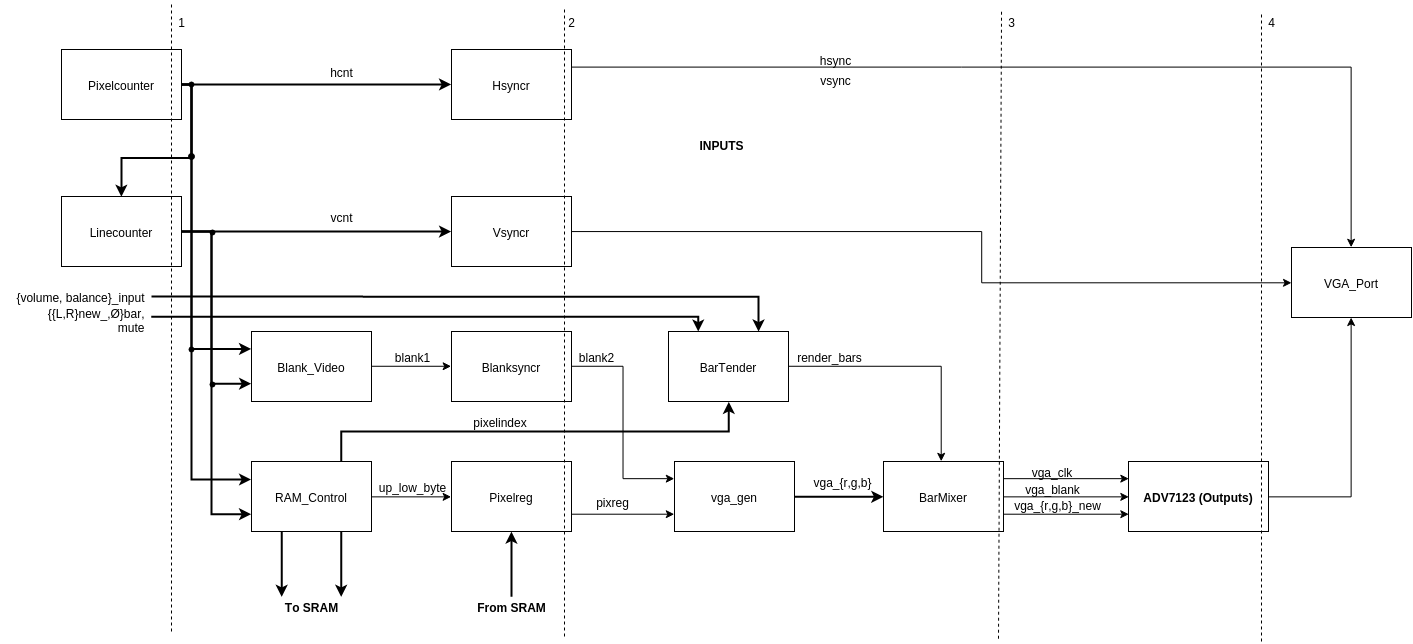
\includegraphics[scale=0.35]{vgadrive.png}
        \caption{Block diagram of vga\_drive}
        \label{fig:vgadrive}
\end{figure}

\begin{figure}[h]
        \caption{List of input signals}
        \label{tab:input}
\begin{tabular}{|r|l|}
        \hline
        \multicolumn{2}{|c|}{Input signals}\\
        \hline
        \multicolumn{1}{|c}{Name} & \multicolumn{1}{c|}{Description} \\
        \hline
        volume\_input & a 4 bit input containing volume information\\
        \cline{1-2}
        \hline
        balance\_input & a 4 bit input containing balance information\\
        \cline{1-2}    
        \hline
        bar & a n bit input containing signal sound input signal level\\
        \cline{1-2}    
        \hline
        new\_bar & a n bit input containing manipulated input signal level\\
        \cline{1-2}    
        \hline
\end{tabular}
\end{figure}

\begin{figure}[h]
        \caption{List of output signals}
        \label{tab:outputs}
\begin{tabular}{|r|l|}     
        \hline
        \multicolumn{2}{|c|}{output signals}\\
        \hline
        \multicolumn{1}{|c}{Name} & \multicolumn{1}{c|}{Description} \\
        \hline
        vga\_clk & clock signal needed for scanning\\
        \cline{1-2}
        \hline
        vga\_blank & a blanking signal for blanking when reseting scan\\
        \cline{1-2}    
        \hline
        vga\_(r,g,b) & three signals containing color information\\
        \cline{1-2}    
        \hline
\end{tabular}
\end{figure}

  \subsection{VGA\_driver:bartender}
  \subsection{VGA\_driver:barmixer}





\chapter{Challenges in the Design and Proposed Approach}\label{ch:challenges}
%\emph{Challenges in the Design and Proposed Approach (Main 2 or 3 challenges and proposed solutions, 1/2 to 1 page per challenge).}

%% Remove the text above

The major problem in the project is the merging of the different modules together
at top level. Most of the modules will be written and debugged separately and
only need minor adjustments before they have been used in a bigger system.
This puts high pressure on this document since a well thought through and described
design hopefully will result in pieces matching together.

A solution is to create and debug all modules and submodules individually
using test benches and waveforms to make sure the modules work exactly as
they are supposed to before putting them all together.

\section{The Logic of Adjusting Volume and Balance}
This is a challenge. It will be solved.


\section{Low Pass Filtering}
Different approaches to making a function for a low pass filter will be considered.

The low pass filter will be a part of the \verb=Analysis= module since it will only be used to refine the displayed power levels. The respective bars rendered on the screen will be delayed by at least 100 ms in order to allow a satisfactory result of the filtering, since there s a need for future values and the filtering is done in real time.

Before implementation, time will be put aside to study and understand the problem further.


\section{Bar Graph Rendering}
Stuff has to be rendered on the screen. This is not an issue, but rendering the right stuff is.



\chapter{User Interface}\label{ch:UI}
%\emph{User Interface (How to control the system + image visualized on the screen).}





The user interface will be able to desplay all the manageable settings on a VGA screen %	\\fotnot{req 3}.
	Ther will in total be four bars. One to indicate the left incomming power, one to indicate the right 
	incoming power, one to indicate the modified left power and one to incidate the modified right power.

	The user interface will also desplay the current volume graduated in dB. The scale goes form -15 dB to +15 dB.







%% Remove the text above


%\appendix
%\chapter{Appendix: System Overview}\label{app:overview}
%\pagenumbering{Roman}
%%\newpage
\begin{figure}[H]
  \centering
  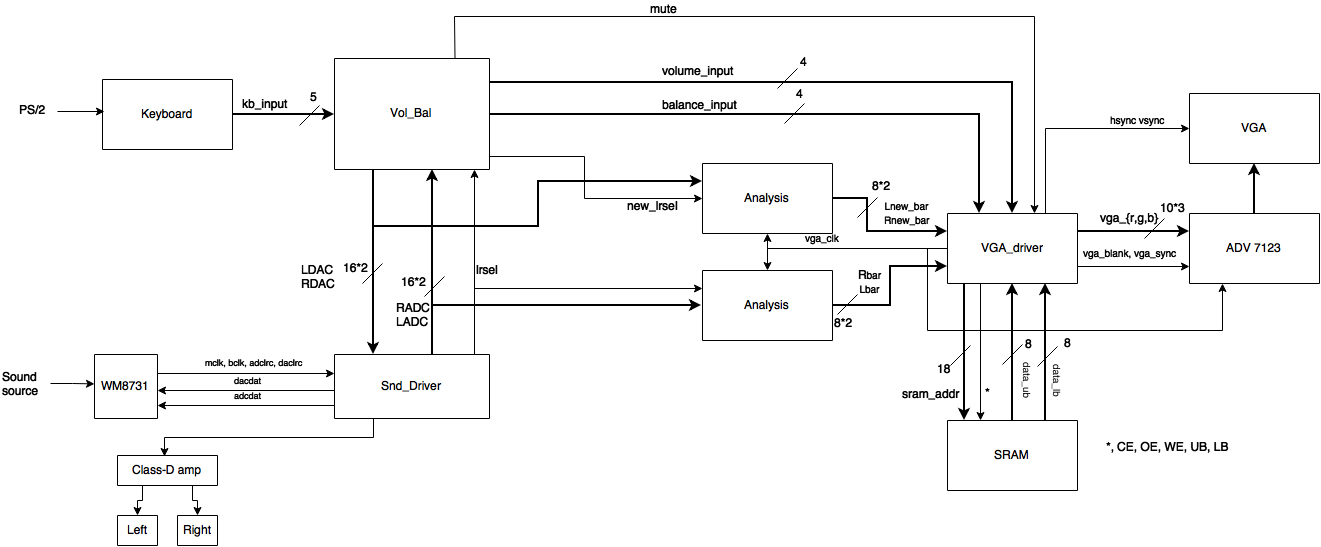
\includegraphics[angle=90, scale=.20]{overview}
%  \caption{This picture is to be redrawn to properly fit a paper layout.}
  \label{fig:hi_overview}
\end{figure}


%% Main Document
\pagestyle{plain}
\setcounter{page}{1}

\section{Introduction}\label{cha:intro}
This is the final report treating the final project in the course
TSIU03 System design. The project was to design and implement a device
used for audio signal processing. 

Using a DE2 board an external audio source can be connected via a
3.5mm port, the signal is then processed by the application and an
image is rendered on a vga screen displaying four signal level bars
representing the left and right channels both before and after
manipulation. There is also two bars displaying the current volume and
balance setting.

The application also accepts input via a ps/2 keyboard used for
setting volume  


\section{Achievements}\label{cha:achievements}
  \subsection{User Noticable Achievements}\label{sec:userachievments}
  \begin{itemize}
\item Remarkably astonishing graphics.
\item Power level indicators for both the input and output sound signal. 
\item The indicators are moving at a smooth rate with absolutely no flickering.
\item Displaying the current volume and balance adjustments made in a user friendly way.
\item Both the minimum and maximum level of adjustments available to the volume and balance is visible to the user.
\item A mute button is shown if the volume is set to be muted.
\item Output sound is sent to a class-D amplifier.
\item Each bar has a peak level indicator.
\item The peak level indicator falls slowly when the power bar is lower than the peak level indicator.
\end{itemize}


  \subsection{Design Challenges}\label{sec:designchallenges}
  \begin{itemize}
\item Use the SRAM to store information about a background picture.
\item Implement a low-pass filter for our signal level indicators. 
\item Bar graph rendering (which pixels to write/blank).
\item The logic of adjusting the volume and balance correctly.
\item Detect each key press only once to prevent drastic changes.
\end{itemize}

\section{System Level Description}\label{cha:syslvl}
\begin{figure}[H]
  \centering
  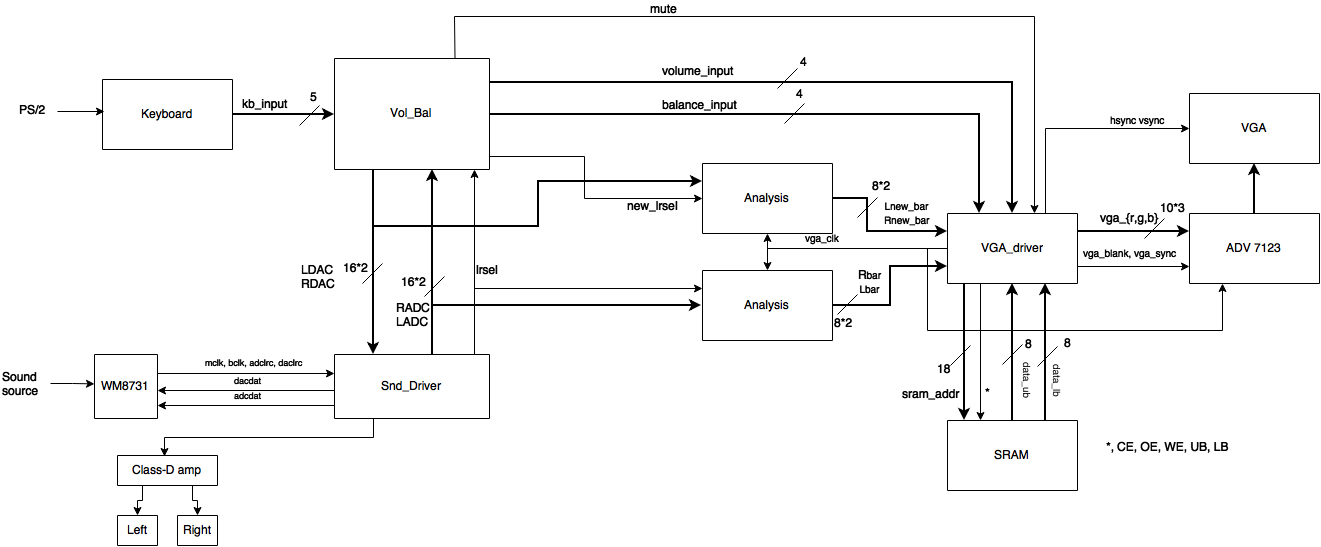
\includegraphics[width=16cm]{overview}
  \caption{G41 Project System Overview}
  \label{fig:overview}
\end{figure}

The project consists of five major modules -- \texttt{Keyboard, Vol\_Bal, Snd\_Driver, Analysis, }and \texttt{VGA\_Driver}. Presented here is an overview of the modules, and more detailed functionality is described in the \citeD.

The system takes, with help of \texttt{Snd\_Driver}, digitally encoded sound from the WM8731 chip. The sound data is passed on to the first instance of \texttt{Analysis} which provides (in order to smoothen the bar movements) low-pass filtered control signals to \texttt{VGA\_Driver:bartender} to assist the rendering of the pre-processing bar graphs done by \texttt{VGA\_Driver} as a whole. The audio data from \texttt{Snd\_Driver} is also passed on to \texttt{Vol\_Bal} which in combination with the control signals from \texttt{Keyboard} adjusts the audio balance %% mjaaa, omformuleras nog
and volume and sends it back to \texttt{Snd\_Driver} which sends signals for the class-D amplifier through the GPIO:s. The adjusted audio is also forked off to a second \texttt{Analysis} instance, which assists the post-processing bar graph rendering.

Whereas \texttt{Keyboard} and \texttt{Analysis} already are fairly small and monolithic modules, and \texttt{Snd\_Driver} and \texttt{Vol\_Bal} consists of three submodules each, \texttt{VGA\_Driver} consists of no less than twelve submodules.

\texttt{Keyboard} handles the PS/2 keyboard user input. The module filters break scan codes (F0$_{16}$, XX$_{16}$) bytewise (11 bit/byte) and compares the XX$_{16}$ byte (iff directly preceeded by F0$_{16}$) to the control key values. This approach will allow the system to respond to the regular keys (ARROW keys and END) as well as corresponding numeric keypad keys as initial E0$_{16}$ bytes are discarded. Upon a registered valid key release, a 5-bit control signal (\verb=kb_input=)is sent for a single clock cycle to \texttt{Vol\_Bal}.

\texttt{Analysis} reads the \verb=ADC= signals and lowpass filters these with a saturation time of approximately 100 ms (4096 clock cycles). These signals are converted to a graph height (in pixels) and passed on to \verb=bar_tender=.

\texttt{Snd\_Driver} have the three submodules \verb=Snd_Driver:{Ctrl,Channel_Mod}= if we count the two instances of \texttt{Channel\_Mod}. These are verbatim copies of \emph{Laboration 4}. The only difference is that the outputs are sent to GPIO pins (and from there via an i2c adapter to the class-D amp) as well as back to the WM8731 codec.

\texttt{Vol\_Bal} consists of the three submodules \verb=Vol_Bal:{Current_Vol_Bal,{Volume,Balance}_Adjustment}=. \verb=Current_Vol_Bal= reads \verb=kb_input= and updates registers representing system levels of volume, balance and mute.
\verb=Volume_Adjustment= adjusts volume according to the volume\_level input from \verb=Current_Vol_Bal=, decreasing amplitude by up to -30 dB in 3 dB decrements, and \verb=Balance_Adjustment= adjusts the audio according to system balance level, resulting in a linear scaling the incoming amplitude. The stronger a channel bias, the higher the signal reduction of the opposing channel. The affected channel loses 1/8 of the amplitude per level of bias.

\texttt{VGA\_Driver} with its submodules handles the rendering of the UI. The module is, in essence, a modified version of the module used in \emph{Laboration 3}. The most significant difference is found in the two new modules \verb=VGA_Driver:Bar_Tender= and \verb=VGA_Driver:Bar_Mixer=. \verb=Bar_Tender= uses the output from \verb=Vol_Bal= and each of the \verb=Analysis= modules along with \verb={h,v}cnt= to calculate which pixel is to be rendered and if it should be rendered from the background image or if to draw it black. The result of the calculations is the control signal \verb=render_bar=. This signal is then passed to \verb=Bar_Mixer=, which is basically a multiplexer, either forwarding the loaded background colors or a blacked out pixel depending on \verb=render_bar= from \verb=Bar_Tender=.


\section{Justification of the Achievements}\label{cha:justice}
%\input{.tex/foo.tex}


\section{User Interface}\label{cha:ui}
The system is controlled by 5 keys on a PS/2-connected keyboard. Down in the table you can see which key that changes what in the system.


\begin{figure}[h]
\centering
%\caption{PS/2 keys and how the input affects the system.}
\begin{tabular}{|c|c|}
\hline
KEY & Function\\ \hline
U ARROW & Volume Increase\\ \hline
L ARROW & Balance Bias Left\\ \hline
D ARROW &  Volume Decrease\\ \hline
R ARROW &  Balance Bias Right\\ \hline
END		&  Mute Volume\\ \hline
\end{tabular}
\caption{PS/2 keys and how the input affects the system.}
\label{fig:scancodes}
\end{figure}


The volume level has eleven diffrent stages, exclusive mute. When the volume is at max, the whole bar will be red, and when the volume is decreased by one the bar will decrease to show the current volume.

The balance level has eighteen diffrent stages. Eight for left balance, eight for right balance and one stage when the signal is equal. When the balance is equal for left and right the only thing you will notice is the bar and divider. But when you for example press the left arrow, the left side will be filled and the outgoing volume on the right will of course decrease.

To indicate that mute is enable you can see one green speaker with a cross to the left side of the picture, and when mute is disable there will only be black. You will also be able to see that the after bars will not show anything, due that nothing is beeing sent out. 

You will be able to see one peak level indicator for each bar, the peak level indicator falls slowly when the power bar is lower than the peak level indicator. With our peak level indicator our user expreience is taken to a whole new level, as you will notice when you use our system you will be overwhelming by the effect.

\begin{figure}[h]
	\centering
        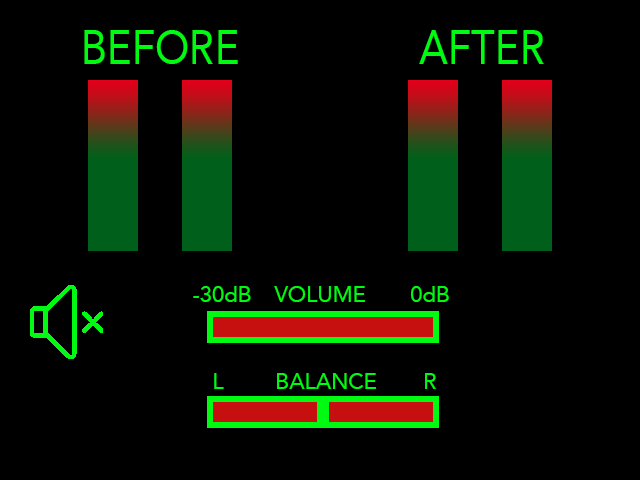
\includegraphics[scale=1]{UI2.png}
       \caption{User interface}
        \label{fig:user interface}
\end{figure}




\section{Improvements}\label{cha:improvements}
The system follows the requirement and design specification quite closely. However there are still possibilities to further develop it into an enjoyable piece. There's a bug with the peak level indicator.  At certain changes, the peak level indicator will disappear and begin falling from the top of the bar, as if it had just rendered a peak that was as big  as the entity of the bar. The peak level indicator, feature wise, could when updated have a slight pause at the peak, so it can be observed more clearly before beginning to drop.

The bars of the sound amplitude are currently a gradient drawn on the background image, being covered by a black bar, to display the amplitude in a gradient bar. However, since it's drawn in the image of the background, the gradient can't change. A possible improvement to the aesthetic of the bar would be rendering the gradient with every time the bar is rendered. Of course this requires quite a bit of back tracking because it's a vastly differnt way to draw bars. 

For clarity, if anyone would ever watch bars to learn anything, the signal bars could have their axis marked with units, thus one could see roughly at what amplitude the peak level indicators stop, for example.

Improvements to the volume and balance bars could include adding more levels. It would be an easy improvement to make, seeing as it's a change that doesn't require going back on decisions already made. The balance bar would of course require a slight change in the background image because of the pre drawn boxes for the balance levels. The volume bar doesn't have the same limitation.

From the keyboard, we currently read the button being released. This helps us avoid problems with the same button being pressed multiple times, or held down. A flaw this causes is that you have to press the button multiple times to cause the effect of it to happen multiple times. If you for example would like to switch the balance fully to the left channel from being fully to the right, that's ten key presses. With clever PS/2 handling, support could be added for a button being held down in order to  repeat the command of that button. This would especially be useful if more leveles were added to the volume and balance levels. 

As an improvemtn, the keyboard could be given control of a lot of variables in the system. For example, the coefficient of the lowering of the peak level indicator., the low pass filtering coefficient (in Analysis). This would give the user more control of the system.

\section{Evaluation of the Project Execution}\label{cha:eval}
\section{Personal Experiences}\label{cha:personalexp}
  \subsection{Niklas}
  
With a well written design the conversion from text to VHDL went super smooth and was therefore very enjoyable. One thing I will take as a lesson is the fact that you should consider which different ways of implementing the same problem there is, consider the pros and cons of each way and from there on pick the most suitable one. 
I definitely had a good time working on this project.
  \subsection{Philip}
   We spent a lot of time on design. We discussed a lot in the group and calculated on much, the whole design was very well thought out and I an had very good control throughout the system. This led to the implementation going very well, and there not being much trouble in assembling the system. This is something I will take with me in life.

  \subsection{Matteus}
  All things considered, the project was enlightening with many valuable lessons. Translating the design into our first prototype was quick and done with ease thanks to our design specification - thus emphasising the importance of preparation and good structuring.

Some specific knowledge learned: Modelsim is a powerful tool in resolving bugs and ensuring correct design implementation; word lengths and overflow are the sources of many problems; timing diagrams are very useful.

As for improving the course - we were advised to not use a certain state machine implementation shown in the lectures.
	

	
  \subsection{Johan}
  The most enjoyable part for me was seeing the shift from design specification to vhdl code. In my head it wouldn't go as easily as it turned out to. If there's anything I wil make sure to learn from, it's going to be writing good design speicifcations. I feel that it should be applicable to other projects.
  \subsection{Oscar}
  Foremost, the project has significantly increased my comprehension of digital circuit design. It has also shown that (which I am sure all of us already knew) that preparation is indeed key to success. Considering my fetish of documentation, I can not truthfully say that the sparse form of documentation has been a favourite of mine, but considering the given time frame, the intention with the project, and the fact that the course runs in parallel with TDDI02, I have to give it a pass. Over all, it has been a greatly enjoyable course.

  \subsection{Erik}
  As previous members have noted the design was very well thought
through and the implementation only differed in minor areas. My
biggest challenge was to operate the software, modelsim especially. I
probably should have payed more attention in the labs on how to
operate it cause getting it started and getting the test-bench working
took almost as long as the testing itself wich felt like a waste of time.


%%% Examples for bibliography

%% Bok
% Bryman, Alan (2002),
% \emph{Samhällsvetenskapliga metoder}.
% Malmö: Liber Ekonomi

%% Antologi
% Florin, Cristina & Johansson, Ulla (1996),
% Tre kulturer – tre historier: Disciplinering i läroverk, flickskolor och folkskolor under 1800-talets senare hälft.
% I S.G. Nordström (red.), \emph{Utbildningshistoria}. Årsböcker i svensk undervisningshistoria, vol. 182.
% Uppsala: Reprocentralen HSC

%% Tidsskrift
% Eriksson, Lisbeth (1999),
% Deltagarna i Kvinnonavet.
% I Susanne Köpsén (red.) \emph{ Motdrag i förort -– ett folkbildningsprojekt i ett mångkulturellt bostadsområde. }
% Linköping: Linköpings universitet. Vuxenutbildarcentrums skriftserie nr. 12/99

%% Fler exempel
% Se Svenska Skrivregler 5.2

%%% Bibliography
%\renewcommand*{\refname}{}
%\addcontentsline{toc}{chapter}{Bibliography}
\renewcommand*{\refname}{References to the Project File}
\begin{thebibliography}{99}\label{cha:refs}

\bibitem{design}
  \href{https://github.com/oscpe262/TSIU03.Project/blob/master/Designspec/designspec.pdf}{
    Group 41 - Design Specification,
    \emph{Linköping},
    2015-10-19.
  }

\bibitem{reqspec}
  \href{https://github.com/oscpe262/TSIU03.Project/blob/master/Kravspec/Kravspecifikation.pdf}{
    Group 41 - Requirement Specification,
    \emph{Linköping},
    2015-09-22.
  }
  
\bibitem{pres}
  \href{https://github.com/oscpe262/TSIU03.Project/blob/master/Presentationer/firstpres.pdf}{
    Group 41 - First Presentation,
    \emph{Linköping},
    2015-10-15.
  }
  
\bibitem{plan}
  \href{https://github.com/oscpe262/TSIU03.Project/blob/master/Projektplan/Project.plan.pdf}{
    Group 41 - Project Plan,
    \emph{Linköping}
    2015-09-24.
  }
  
%\bibitem{vhdldummy}
%  \href{https://github.com/oscpe262/TSIU03.Project/blob/master/<directory>/<filename>}{
%    ModuleName,
%    \texttt{filename.vhd}
%  }
  
\end{thebibliography}
\let\thefootnote\relax\footnote{All documents available at \url{https://github.com/oscpe262/TSIU03.Project}. The references in the PDF version of this document are hyperlinks to the document listed. The PDF can be downloaded at: \\\url{https://github.com/oscpe262/TSIU03.Project/blob/master/Projektrapport/report.pdf}.}




\end{document}
